\documentclass{article}
\usepackage{amsmath,amssymb,booktabs,longtable,tikz,graphicx}
\usepackage[margin=16mm]{geometry}
\begin{document}
\section*{Six-dimensional $\phi^3$: two-loop three-point counterterms}
Fixed external labels; amputated connected 1PI; $g^5$ factored out. Local integrals remain symbolic.
\[S_{int}=g\phi^3/3!,\quad v_3=-g,\quad C_\gamma=-t_\gamma\bar R_\gamma,\quad R_G=(1-t_G)\bar R_G.\]
\[t_2: \deg(p)\le2,\qquad t_3: \deg(p_1,p_2)=0.\]
\[K_m=\int D(q)^2,\quad K_z=\int[-D(q)^3+\tfrac46q^2D(q)^4],\quad K_3=\int D(q)^3.\]
\[v_{2m}=-g^2K_m/2,\quad v_{2z}(p)=-g^2K_zp^2/2,\quad v_{3,1}=+g^3K_3.\]
\begin{center}\resizebox{\textwidth}{!}{\begin{tabular}{lccccccccccc}
\toprule
Graph & I & M12 & M13 & M23 & Z12 & Z13 & Z23 & G1 & G2 & G3 & C3L2 \\\midrule
L2E3G1 & $-1/2$ & $0$ & $0$ & $0$ & $0$ & $0$ & $0$ & $0$ & $0$ & $0$ & $1/2T_0\,I$ \\
L2E3G2 & $-1$ & $0$ & $0$ & $0$ & $0$ & $0$ & $0$ & $1$ & $0$ & $0$ & $-1T_0\,G1+1T_0\,I$ \\
L2E3G3 & $-1$ & $0$ & $0$ & $0$ & $0$ & $0$ & $0$ & $0$ & $1$ & $0$ & $-1T_0\,G2+1T_0\,I$ \\
L2E3G4 & $-1/2$ & $1/2$ & $0$ & $0$ & $1/2$ & $0$ & $0$ & $0$ & $0$ & $0$ & $-1/2T_0\,M12-1/2T_0\,Z12+1/2T_0\,I$ \\
L2E3G5 & $-1$ & $0$ & $0$ & $0$ & $0$ & $0$ & $0$ & $0$ & $0$ & $1$ & $-1T_0\,G3+1T_0\,I$ \\
L2E3G6 & $-1/2$ & $0$ & $1/2$ & $0$ & $0$ & $1/2$ & $0$ & $0$ & $0$ & $0$ & $-1/2T_0\,M13-1/2T_0\,Z13+1/2T_0\,I$ \\
L2E3G7 & $-1/2$ & $0$ & $0$ & $1/2$ & $0$ & $0$ & $1/2$ & $0$ & $0$ & $0$ & $-1/2T_0\,M23-1/2T_0\,Z23+1/2T_0\,I$ \\
\bottomrule\end{tabular}}\end{center}
Every cell is checked by two independent algorithms. Zeros are structural, not approximate.
External reference diagrams remain unavailable. The 162-case research ledger records 24 strict analytic, 48 empirical and 90 unresolved cases.
\subsection*{L2E3G1}
% shared-layout-id: 2c3c3c7ad6b2c58ae6bfca4498d8cd27c0ce26dbb417fa4068cd0397563b27c8
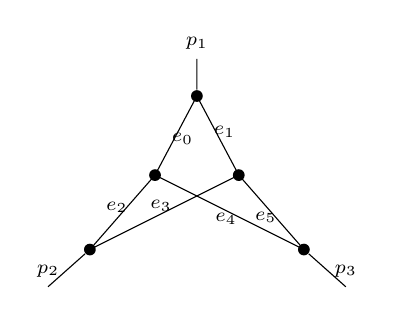
\begin{tikzpicture}[scale=.65,every node/.style={font=\scriptsize}]
\node[circle,fill,inner sep=1.5pt] (v0) at (3.27272727,4.18181818) {};
\node[circle,fill,inner sep=1.5pt] (v1) at (1.18181818,1.18181818) {};
\node[circle,fill,inner sep=1.5pt] (v2) at (5.36363636,1.18181818) {};
\node[circle,fill,inner sep=1.5pt] (v3) at (2.45454545,2.63636364) {};
\node[circle,fill,inner sep=1.5pt] (v4) at (4.09090909,2.63636364) {};
\draw[black] (3.27272727,4.18181818) .. controls (3.00000000,3.66666667) and (2.72727273,3.15151515) .. (2.45454545,2.63636364);
\node at (2.99218733,3.34103451) {$e_{0}$};
\draw[black] (3.27272727,4.18181818) .. controls (3.54545455,3.66666667) and (3.81818182,3.15151515) .. (4.09090909,2.63636364);
\node at (3.81036915,3.47714730) {$e_{1}$};
\draw[black] (1.18181818,1.18181818) .. controls (1.60606061,1.66666667) and (2.03030303,2.15151515) .. (2.45454545,2.63636364);
\node at (1.70871612,2.00487340) {$e_{2}$};
\draw[black] (1.18181818,1.18181818) .. controls (2.15151515,1.66666667) and (3.12121212,2.15151515) .. (4.09090909,2.63636364);
\node at (2.57131439,2.03918941) {$e_{3}$};
\draw[black] (5.36363636,1.18181818) .. controls (4.39393939,1.66666667) and (3.42424242,2.15151515) .. (2.45454545,2.63636364);
\node at (3.84404166,1.77899241) {$e_{4}$};
\draw[black] (5.36363636,1.18181818) .. controls (4.93939394,1.66666667) and (4.51515152,2.15151515) .. (4.09090909,2.63636364);
\node at (4.61780703,1.81330842) {$e_{5}$};
\draw (v0) -- (3.27272727,4.90909091) node[above] {$p_{1}$};
\draw (v1) -- (0.36363636,0.45454545) node[above] {$p_{2}$};
\draw (v2) -- (6.18181818,0.45454545) node[above] {$p_{3}$};
\end{tikzpicture}
Positive weight: $1/S=1/2$.
\begin{itemize}
\item I: $- 1/2$
\item C3L2: $1/2 T_0\,I$
\end{itemize}
\subsection*{L2E3G2}
% shared-layout-id: 3e3a80323aa641544cbf16c259761899566e04fc4f7396c676c03315cd0e9f62
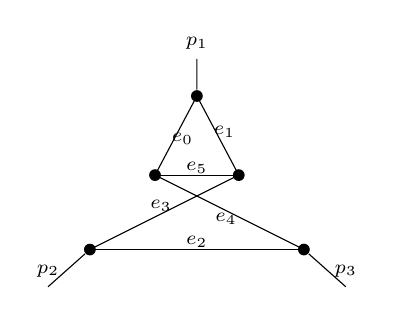
\begin{tikzpicture}[scale=.65,every node/.style={font=\scriptsize}]
\node[circle,fill,inner sep=1.5pt] (v0) at (3.27272727,4.18181818) {};
\node[circle,fill,inner sep=1.5pt] (v1) at (1.18181818,1.18181818) {};
\node[circle,fill,inner sep=1.5pt] (v2) at (5.36363636,1.18181818) {};
\node[circle,fill,inner sep=1.5pt] (v3) at (2.45454545,2.63636364) {};
\node[circle,fill,inner sep=1.5pt] (v4) at (4.09090909,2.63636364) {};
\draw[black] (3.27272727,4.18181818) .. controls (3.00000000,3.66666667) and (2.72727273,3.15151515) .. (2.45454545,2.63636364);
\node at (2.99218733,3.34103451) {$e_{0}$};
\draw[black] (3.27272727,4.18181818) .. controls (3.54545455,3.66666667) and (3.81818182,3.15151515) .. (4.09090909,2.63636364);
\node at (3.81036915,3.47714730) {$e_{1}$};
\draw[black] (1.18181818,1.18181818) .. controls (2.57575758,1.18181818) and (3.96969697,1.18181818) .. (5.36363636,1.18181818);
\node at (3.27272727,1.32727273) {$e_{2}$};
\draw[black] (1.18181818,1.18181818) .. controls (2.15151515,1.66666667) and (3.12121212,2.15151515) .. (4.09090909,2.63636364);
\node at (2.57131439,2.03918941) {$e_{3}$};
\draw[black] (5.36363636,1.18181818) .. controls (4.39393939,1.66666667) and (3.42424242,2.15151515) .. (2.45454545,2.63636364);
\node at (3.84404166,1.77899241) {$e_{4}$};
\draw[black] (2.45454545,2.63636364) .. controls (3.00000000,2.63636364) and (3.54545455,2.63636364) .. (4.09090909,2.63636364);
\node at (3.27272727,2.78181818) {$e_{5}$};
\draw (v0) -- (3.27272727,4.90909091) node[above] {$p_{1}$};
\draw (v1) -- (0.36363636,0.45454545) node[above] {$p_{2}$};
\draw (v2) -- (6.18181818,0.45454545) node[above] {$p_{3}$};
\end{tikzpicture}
Positive weight: $1/S=1$.
\begin{itemize}
\item I: $- 1$
\item G1: $1$
\item C3L2: $- 1 T_0\,G1 + 1 T_0\,I$
\end{itemize}
\subsection*{L2E3G3}
% shared-layout-id: 3a2826995eb0d1e1511b7a015eb9cc768b0bc8228064c5faa862a83588f5f42e
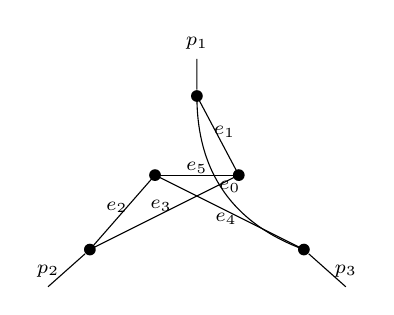
\begin{tikzpicture}[scale=.65,every node/.style={font=\scriptsize}]
\node[circle,fill,inner sep=1.5pt] (v0) at (3.27272727,4.18181818) {};
\node[circle,fill,inner sep=1.5pt] (v1) at (1.18181818,1.18181818) {};
\node[circle,fill,inner sep=1.5pt] (v2) at (5.36363636,1.18181818) {};
\node[circle,fill,inner sep=1.5pt] (v3) at (2.45454545,2.63636364) {};
\node[circle,fill,inner sep=1.5pt] (v4) at (4.09090909,2.63636364) {};
\draw[black] (3.27272727,4.18181818) .. controls (3.27360156,2.69666077) and (3.97057125,1.69666077) .. (5.36363636,1.18181818);
\node at (3.91544090,2.40111997) {$e_{0}$};
\draw[black] (3.27272727,4.18181818) .. controls (3.54545455,3.66666667) and (3.81818182,3.15151515) .. (4.09090909,2.63636364);
\node at (3.81036915,3.47714730) {$e_{1}$};
\draw[black] (1.18181818,1.18181818) .. controls (1.60606061,1.66666667) and (2.03030303,2.15151515) .. (2.45454545,2.63636364);
\node at (1.70871612,2.00487340) {$e_{2}$};
\draw[black] (1.18181818,1.18181818) .. controls (2.15151515,1.66666667) and (3.12121212,2.15151515) .. (4.09090909,2.63636364);
\node at (2.57131439,2.03918941) {$e_{3}$};
\draw[black] (5.36363636,1.18181818) .. controls (4.39393939,1.66666667) and (3.42424242,2.15151515) .. (2.45454545,2.63636364);
\node at (3.84404166,1.77899241) {$e_{4}$};
\draw[black] (2.45454545,2.63636364) .. controls (3.00000000,2.63636364) and (3.54545455,2.63636364) .. (4.09090909,2.63636364);
\node at (3.27272727,2.78181818) {$e_{5}$};
\draw (v0) -- (3.27272727,4.90909091) node[above] {$p_{1}$};
\draw (v1) -- (0.36363636,0.45454545) node[above] {$p_{2}$};
\draw (v2) -- (6.18181818,0.45454545) node[above] {$p_{3}$};
\end{tikzpicture}
Positive weight: $1/S=1$.
\begin{itemize}
\item I: $- 1$
\item G2: $1$
\item C3L2: $- 1 T_0\,G2 + 1 T_0\,I$
\end{itemize}
\subsection*{L2E3G4}
% shared-layout-id: 069d9e186a0cc38bc97522c608115273a4208bf6321c683df74499e764ca36f3
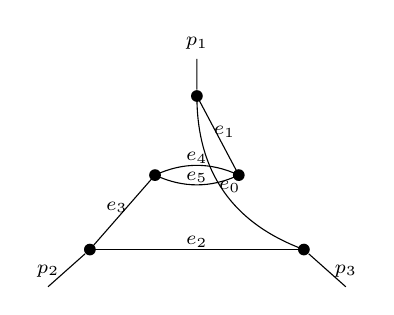
\begin{tikzpicture}[scale=.65,every node/.style={font=\scriptsize}]
\node[circle,fill,inner sep=1.5pt] (v0) at (3.27272727,4.18181818) {};
\node[circle,fill,inner sep=1.5pt] (v1) at (1.18181818,1.18181818) {};
\node[circle,fill,inner sep=1.5pt] (v2) at (5.36363636,1.18181818) {};
\node[circle,fill,inner sep=1.5pt] (v3) at (2.45454545,2.63636364) {};
\node[circle,fill,inner sep=1.5pt] (v4) at (4.09090909,2.63636364) {};
\draw[black] (3.27272727,4.18181818) .. controls (3.27360156,2.69666077) and (3.97057125,1.69666077) .. (5.36363636,1.18181818);
\node at (3.91544090,2.40111997) {$e_{0}$};
\draw[black] (3.27272727,4.18181818) .. controls (3.54545455,3.66666667) and (3.81818182,3.15151515) .. (4.09090909,2.63636364);
\node at (3.81036915,3.47714730) {$e_{1}$};
\draw[black] (1.18181818,1.18181818) .. controls (2.57575758,1.18181818) and (3.96969697,1.18181818) .. (5.36363636,1.18181818);
\node at (3.27272727,1.32727273) {$e_{2}$};
\draw[black] (1.18181818,1.18181818) .. controls (1.60606061,1.66666667) and (2.03030303,2.15151515) .. (2.45454545,2.63636364);
\node at (1.70871612,2.00487340) {$e_{3}$};
\draw[black] (2.45454545,2.63636364) .. controls (3.00000000,2.89090909) and (3.54545455,2.89090909) .. (4.09090909,2.63636364);
\node at (3.27272727,2.97272727) {$e_{4}$};
\draw[black] (2.45454545,2.63636364) .. controls (3.00000000,2.38181818) and (3.54545455,2.38181818) .. (4.09090909,2.63636364);
\node at (3.27272727,2.59090909) {$e_{5}$};
\draw (v0) -- (3.27272727,4.90909091) node[above] {$p_{1}$};
\draw (v1) -- (0.36363636,0.45454545) node[above] {$p_{2}$};
\draw (v2) -- (6.18181818,0.45454545) node[above] {$p_{3}$};
\end{tikzpicture}
Positive weight: $1/S=1/2$.
\begin{itemize}
\item I: $- 1/2$
\item M12: $1/2$
\item Z12: $1/2$
\item C3L2: $- 1/2 T_0\,M12 - 1/2 T_0\,Z12 + 1/2 T_0\,I$
\end{itemize}
\subsection*{L2E3G5}
% shared-layout-id: 3fab0242e6f5f84258bf8164bcb645886eb580f2f85516b90321fc55e0badd50
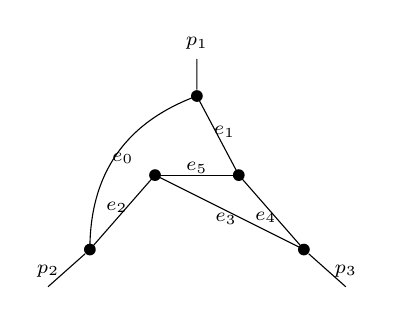
\begin{tikzpicture}[scale=.65,every node/.style={font=\scriptsize}]
\node[circle,fill,inner sep=1.5pt] (v0) at (3.27272727,4.18181818) {};
\node[circle,fill,inner sep=1.5pt] (v1) at (1.18181818,1.18181818) {};
\node[circle,fill,inner sep=1.5pt] (v2) at (5.36363636,1.18181818) {};
\node[circle,fill,inner sep=1.5pt] (v3) at (2.45454545,2.63636364) {};
\node[circle,fill,inner sep=1.5pt] (v4) at (4.09090909,2.63636364) {};
\draw[black] (3.27272727,4.18181818) .. controls (1.87966216,3.66697559) and (1.18269246,2.66697559) .. (1.18181818,1.18181818);
\node at (1.82453181,2.96251640) {$e_{0}$};
\draw[black] (3.27272727,4.18181818) .. controls (3.54545455,3.66666667) and (3.81818182,3.15151515) .. (4.09090909,2.63636364);
\node at (3.81036915,3.47714730) {$e_{1}$};
\draw[black] (1.18181818,1.18181818) .. controls (1.60606061,1.66666667) and (2.03030303,2.15151515) .. (2.45454545,2.63636364);
\node at (1.70871612,2.00487340) {$e_{2}$};
\draw[black] (5.36363636,1.18181818) .. controls (4.39393939,1.66666667) and (3.42424242,2.15151515) .. (2.45454545,2.63636364);
\node at (3.84404166,1.77899241) {$e_{3}$};
\draw[black] (5.36363636,1.18181818) .. controls (4.93939394,1.66666667) and (4.51515152,2.15151515) .. (4.09090909,2.63636364);
\node at (4.61780703,1.81330842) {$e_{4}$};
\draw[black] (2.45454545,2.63636364) .. controls (3.00000000,2.63636364) and (3.54545455,2.63636364) .. (4.09090909,2.63636364);
\node at (3.27272727,2.78181818) {$e_{5}$};
\draw (v0) -- (3.27272727,4.90909091) node[above] {$p_{1}$};
\draw (v1) -- (0.36363636,0.45454545) node[above] {$p_{2}$};
\draw (v2) -- (6.18181818,0.45454545) node[above] {$p_{3}$};
\end{tikzpicture}
Positive weight: $1/S=1$.
\begin{itemize}
\item I: $- 1$
\item G3: $1$
\item C3L2: $- 1 T_0\,G3 + 1 T_0\,I$
\end{itemize}
\subsection*{L2E3G6}
% shared-layout-id: f41709cd06f5cfc22852e804da6c56c5a8b895d3e552cd04a3e609498a3534c2
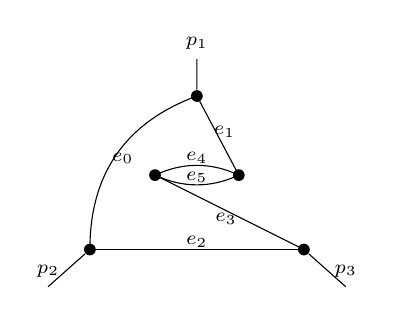
\begin{tikzpicture}[scale=.65,every node/.style={font=\scriptsize}]
\node[circle,fill,inner sep=1.5pt] (v0) at (3.27272727,4.18181818) {};
\node[circle,fill,inner sep=1.5pt] (v1) at (1.18181818,1.18181818) {};
\node[circle,fill,inner sep=1.5pt] (v2) at (5.36363636,1.18181818) {};
\node[circle,fill,inner sep=1.5pt] (v3) at (2.45454545,2.63636364) {};
\node[circle,fill,inner sep=1.5pt] (v4) at (4.09090909,2.63636364) {};
\draw[black] (3.27272727,4.18181818) .. controls (1.87966216,3.66697559) and (1.18269246,2.66697559) .. (1.18181818,1.18181818);
\node at (1.82453181,2.96251640) {$e_{0}$};
\draw[black] (3.27272727,4.18181818) .. controls (3.54545455,3.66666667) and (3.81818182,3.15151515) .. (4.09090909,2.63636364);
\node at (3.81036915,3.47714730) {$e_{1}$};
\draw[black] (1.18181818,1.18181818) .. controls (2.57575758,1.18181818) and (3.96969697,1.18181818) .. (5.36363636,1.18181818);
\node at (3.27272727,1.32727273) {$e_{2}$};
\draw[black] (5.36363636,1.18181818) .. controls (4.39393939,1.66666667) and (3.42424242,2.15151515) .. (2.45454545,2.63636364);
\node at (3.84404166,1.77899241) {$e_{3}$};
\draw[black] (2.45454545,2.63636364) .. controls (3.00000000,2.89090909) and (3.54545455,2.89090909) .. (4.09090909,2.63636364);
\node at (3.27272727,2.97272727) {$e_{4}$};
\draw[black] (2.45454545,2.63636364) .. controls (3.00000000,2.38181818) and (3.54545455,2.38181818) .. (4.09090909,2.63636364);
\node at (3.27272727,2.59090909) {$e_{5}$};
\draw (v0) -- (3.27272727,4.90909091) node[above] {$p_{1}$};
\draw (v1) -- (0.36363636,0.45454545) node[above] {$p_{2}$};
\draw (v2) -- (6.18181818,0.45454545) node[above] {$p_{3}$};
\end{tikzpicture}
Positive weight: $1/S=1/2$.
\begin{itemize}
\item I: $- 1/2$
\item M13: $1/2$
\item Z13: $1/2$
\item C3L2: $- 1/2 T_0\,M13 - 1/2 T_0\,Z13 + 1/2 T_0\,I$
\end{itemize}
\subsection*{L2E3G7}
% shared-layout-id: 577a674b15833eda4c7c4b940eb1f8d28e047d04c3e4793536af9359343c495d
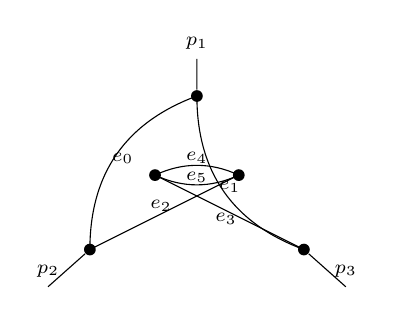
\begin{tikzpicture}[scale=.65,every node/.style={font=\scriptsize}]
\node[circle,fill,inner sep=1.5pt] (v0) at (3.27272727,4.18181818) {};
\node[circle,fill,inner sep=1.5pt] (v1) at (1.18181818,1.18181818) {};
\node[circle,fill,inner sep=1.5pt] (v2) at (5.36363636,1.18181818) {};
\node[circle,fill,inner sep=1.5pt] (v3) at (2.45454545,2.63636364) {};
\node[circle,fill,inner sep=1.5pt] (v4) at (4.09090909,2.63636364) {};
\draw[black] (3.27272727,4.18181818) .. controls (1.87966216,3.66697559) and (1.18269246,2.66697559) .. (1.18181818,1.18181818);
\node at (1.82453181,2.96251640) {$e_{0}$};
\draw[black] (3.27272727,4.18181818) .. controls (3.27360156,2.69666077) and (3.97057125,1.69666077) .. (5.36363636,1.18181818);
\node at (3.91544090,2.40111997) {$e_{1}$};
\draw[black] (1.18181818,1.18181818) .. controls (2.15151515,1.66666667) and (3.12121212,2.15151515) .. (4.09090909,2.63636364);
\node at (2.57131439,2.03918941) {$e_{2}$};
\draw[black] (5.36363636,1.18181818) .. controls (4.39393939,1.66666667) and (3.42424242,2.15151515) .. (2.45454545,2.63636364);
\node at (3.84404166,1.77899241) {$e_{3}$};
\draw[black] (2.45454545,2.63636364) .. controls (3.00000000,2.89090909) and (3.54545455,2.89090909) .. (4.09090909,2.63636364);
\node at (3.27272727,2.97272727) {$e_{4}$};
\draw[black] (2.45454545,2.63636364) .. controls (3.00000000,2.38181818) and (3.54545455,2.38181818) .. (4.09090909,2.63636364);
\node at (3.27272727,2.59090909) {$e_{5}$};
\draw (v0) -- (3.27272727,4.90909091) node[above] {$p_{1}$};
\draw (v1) -- (0.36363636,0.45454545) node[above] {$p_{2}$};
\draw (v2) -- (6.18181818,0.45454545) node[above] {$p_{3}$};
\end{tikzpicture}
Positive weight: $1/S=1/2$.
\begin{itemize}
\item I: $- 1/2$
\item M23: $1/2$
\item Z23: $1/2$
\item C3L2: $- 1/2 T_0\,M23 - 1/2 T_0\,Z23 + 1/2 T_0\,I$
\end{itemize}
\section*{Counterterm host graphs}
\subsection*{M12}
% shared-layout-id: 6c3e193b4cd76280b64248b897d15e9e6d37f6ed9913a968e4cb8175cdb3f858
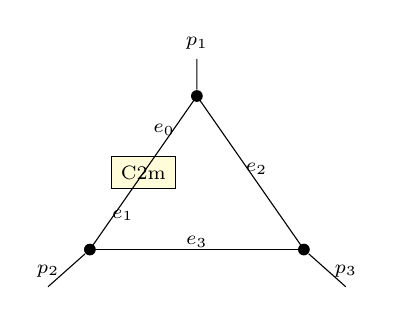
\begin{tikzpicture}[scale=.65,every node/.style={font=\scriptsize}]
\node[rectangle,draw,fill=yellow!15] (v0) at (2.22727273,2.68181818) {C2m};
\node[circle,fill,inner sep=1.5pt] (v1) at (3.27272727,4.18181818) {};
\node[circle,fill,inner sep=1.5pt] (v2) at (1.18181818,1.18181818) {};
\node[circle,fill,inner sep=1.5pt] (v3) at (5.36363636,1.18181818) {};
\draw[black] (2.22727273,2.68181818) .. controls (2.57575758,3.18181818) and (2.92424242,3.68181818) .. (3.27272727,4.18181818);
\node at (2.63066936,3.51498802) {$e_{0}$};
\draw[black] (2.22727273,2.68181818) .. controls (1.87878788,2.18181818) and (1.53030303,1.68181818) .. (1.18181818,1.18181818);
\node at (1.82387610,1.84864834) {$e_{1}$};
\draw[black] (3.27272727,4.18181818) .. controls (3.96969697,3.18181818) and (4.66666667,2.18181818) .. (5.36363636,1.18181818);
\node at (4.43751246,2.76498802) {$e_{2}$};
\draw[black] (1.18181818,1.18181818) .. controls (2.57575758,1.18181818) and (3.96969697,1.18181818) .. (5.36363636,1.18181818);
\node at (3.27272727,1.32727273) {$e_{3}$};
\draw (v1) -- (3.27272727,4.90909091) node[above] {$p_{1}$};
\draw (v2) -- (0.36363636,0.45454545) node[above] {$p_{2}$};
\draw (v3) -- (6.18181818,0.45454545) node[above] {$p_{3}$};
\end{tikzpicture}
\subsection*{M13}
% shared-layout-id: 3f20853e18df856a6bb8a73f96c41665fc923b497a1f67ffbb38737dfd83bd90
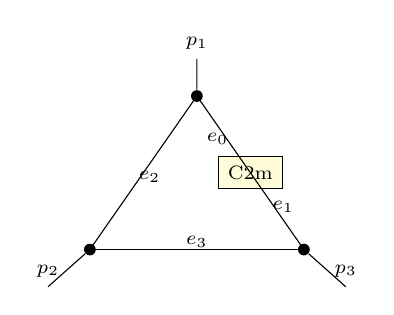
\begin{tikzpicture}[scale=.65,every node/.style={font=\scriptsize}]
\node[rectangle,draw,fill=yellow!15] (v0) at (4.31818182,2.68181818) {C2m};
\node[circle,fill,inner sep=1.5pt] (v1) at (3.27272727,4.18181818) {};
\node[circle,fill,inner sep=1.5pt] (v2) at (1.18181818,1.18181818) {};
\node[circle,fill,inner sep=1.5pt] (v3) at (5.36363636,1.18181818) {};
\draw[black] (4.31818182,2.68181818) .. controls (3.96969697,3.18181818) and (3.62121212,3.68181818) .. (3.27272727,4.18181818);
\node at (3.67612390,3.34864834) {$e_{0}$};
\draw[black] (4.31818182,2.68181818) .. controls (4.66666667,2.18181818) and (5.01515152,1.68181818) .. (5.36363636,1.18181818);
\node at (4.96023973,2.01498802) {$e_{1}$};
\draw[black] (3.27272727,4.18181818) .. controls (2.57575758,3.18181818) and (1.87878788,2.18181818) .. (1.18181818,1.18181818);
\node at (2.34660337,2.59864834) {$e_{2}$};
\draw[black] (1.18181818,1.18181818) .. controls (2.57575758,1.18181818) and (3.96969697,1.18181818) .. (5.36363636,1.18181818);
\node at (3.27272727,1.32727273) {$e_{3}$};
\draw (v1) -- (3.27272727,4.90909091) node[above] {$p_{1}$};
\draw (v2) -- (0.36363636,0.45454545) node[above] {$p_{2}$};
\draw (v3) -- (6.18181818,0.45454545) node[above] {$p_{3}$};
\end{tikzpicture}
\subsection*{M23}
% shared-layout-id: 52efb286d12d2448c23a939b877f5593a4c314376d508b42c64438596ce96ba6
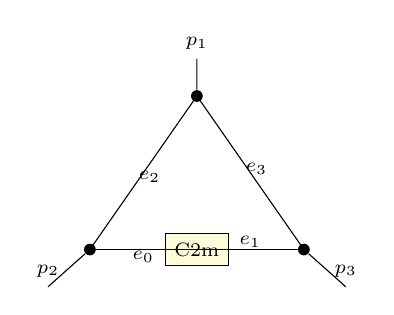
\begin{tikzpicture}[scale=.65,every node/.style={font=\scriptsize}]
\node[rectangle,draw,fill=yellow!15] (v0) at (3.27272727,1.18181818) {C2m};
\node[circle,fill,inner sep=1.5pt] (v1) at (3.27272727,4.18181818) {};
\node[circle,fill,inner sep=1.5pt] (v2) at (1.18181818,1.18181818) {};
\node[circle,fill,inner sep=1.5pt] (v3) at (5.36363636,1.18181818) {};
\draw[black] (3.27272727,1.18181818) .. controls (2.57575758,1.18181818) and (1.87878788,1.18181818) .. (1.18181818,1.18181818);
\node at (2.22727273,1.03636364) {$e_{0}$};
\draw[black] (3.27272727,1.18181818) .. controls (3.96969697,1.18181818) and (4.66666667,1.18181818) .. (5.36363636,1.18181818);
\node at (4.31818182,1.32727273) {$e_{1}$};
\draw[black] (3.27272727,4.18181818) .. controls (2.57575758,3.18181818) and (1.87878788,2.18181818) .. (1.18181818,1.18181818);
\node at (2.34660337,2.59864834) {$e_{2}$};
\draw[black] (3.27272727,4.18181818) .. controls (3.96969697,3.18181818) and (4.66666667,2.18181818) .. (5.36363636,1.18181818);
\node at (4.43751246,2.76498802) {$e_{3}$};
\draw (v1) -- (3.27272727,4.90909091) node[above] {$p_{1}$};
\draw (v2) -- (0.36363636,0.45454545) node[above] {$p_{2}$};
\draw (v3) -- (6.18181818,0.45454545) node[above] {$p_{3}$};
\end{tikzpicture}
\subsection*{Z12}
% shared-layout-id: 642e91b7684097f8f3a8c8da32df37187f955f93f4430b7dd412986ef9cda36b
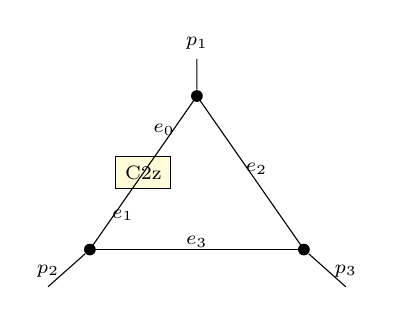
\begin{tikzpicture}[scale=.65,every node/.style={font=\scriptsize}]
\node[rectangle,draw,fill=yellow!15] (v0) at (2.22727273,2.68181818) {C2z};
\node[circle,fill,inner sep=1.5pt] (v1) at (3.27272727,4.18181818) {};
\node[circle,fill,inner sep=1.5pt] (v2) at (1.18181818,1.18181818) {};
\node[circle,fill,inner sep=1.5pt] (v3) at (5.36363636,1.18181818) {};
\draw[black] (2.22727273,2.68181818) .. controls (2.57575758,3.18181818) and (2.92424242,3.68181818) .. (3.27272727,4.18181818);
\node at (2.63066936,3.51498802) {$e_{0}$};
\draw[black] (2.22727273,2.68181818) .. controls (1.87878788,2.18181818) and (1.53030303,1.68181818) .. (1.18181818,1.18181818);
\node at (1.82387610,1.84864834) {$e_{1}$};
\draw[black] (3.27272727,4.18181818) .. controls (3.96969697,3.18181818) and (4.66666667,2.18181818) .. (5.36363636,1.18181818);
\node at (4.43751246,2.76498802) {$e_{2}$};
\draw[black] (1.18181818,1.18181818) .. controls (2.57575758,1.18181818) and (3.96969697,1.18181818) .. (5.36363636,1.18181818);
\node at (3.27272727,1.32727273) {$e_{3}$};
\draw (v1) -- (3.27272727,4.90909091) node[above] {$p_{1}$};
\draw (v2) -- (0.36363636,0.45454545) node[above] {$p_{2}$};
\draw (v3) -- (6.18181818,0.45454545) node[above] {$p_{3}$};
\end{tikzpicture}
\subsection*{Z13}
% shared-layout-id: 84a542d962fdab1f25ab86d210f52dba5cf069e01e77fff268e8eca8249176ae
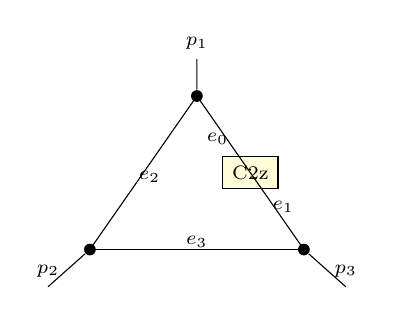
\begin{tikzpicture}[scale=.65,every node/.style={font=\scriptsize}]
\node[rectangle,draw,fill=yellow!15] (v0) at (4.31818182,2.68181818) {C2z};
\node[circle,fill,inner sep=1.5pt] (v1) at (3.27272727,4.18181818) {};
\node[circle,fill,inner sep=1.5pt] (v2) at (1.18181818,1.18181818) {};
\node[circle,fill,inner sep=1.5pt] (v3) at (5.36363636,1.18181818) {};
\draw[black] (4.31818182,2.68181818) .. controls (3.96969697,3.18181818) and (3.62121212,3.68181818) .. (3.27272727,4.18181818);
\node at (3.67612390,3.34864834) {$e_{0}$};
\draw[black] (4.31818182,2.68181818) .. controls (4.66666667,2.18181818) and (5.01515152,1.68181818) .. (5.36363636,1.18181818);
\node at (4.96023973,2.01498802) {$e_{1}$};
\draw[black] (3.27272727,4.18181818) .. controls (2.57575758,3.18181818) and (1.87878788,2.18181818) .. (1.18181818,1.18181818);
\node at (2.34660337,2.59864834) {$e_{2}$};
\draw[black] (1.18181818,1.18181818) .. controls (2.57575758,1.18181818) and (3.96969697,1.18181818) .. (5.36363636,1.18181818);
\node at (3.27272727,1.32727273) {$e_{3}$};
\draw (v1) -- (3.27272727,4.90909091) node[above] {$p_{1}$};
\draw (v2) -- (0.36363636,0.45454545) node[above] {$p_{2}$};
\draw (v3) -- (6.18181818,0.45454545) node[above] {$p_{3}$};
\end{tikzpicture}
\subsection*{Z23}
% shared-layout-id: 3f7cbc2982556b4645667d72c6b66133942ffe7f050fab24bb1e9b9c2c231845
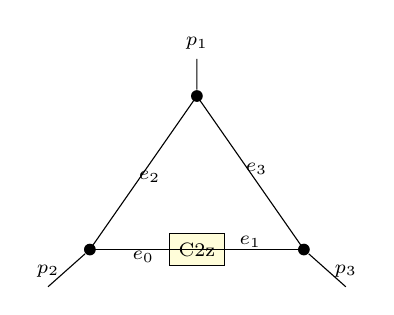
\begin{tikzpicture}[scale=.65,every node/.style={font=\scriptsize}]
\node[rectangle,draw,fill=yellow!15] (v0) at (3.27272727,1.18181818) {C2z};
\node[circle,fill,inner sep=1.5pt] (v1) at (3.27272727,4.18181818) {};
\node[circle,fill,inner sep=1.5pt] (v2) at (1.18181818,1.18181818) {};
\node[circle,fill,inner sep=1.5pt] (v3) at (5.36363636,1.18181818) {};
\draw[black] (3.27272727,1.18181818) .. controls (2.57575758,1.18181818) and (1.87878788,1.18181818) .. (1.18181818,1.18181818);
\node at (2.22727273,1.03636364) {$e_{0}$};
\draw[black] (3.27272727,1.18181818) .. controls (3.96969697,1.18181818) and (4.66666667,1.18181818) .. (5.36363636,1.18181818);
\node at (4.31818182,1.32727273) {$e_{1}$};
\draw[black] (3.27272727,4.18181818) .. controls (2.57575758,3.18181818) and (1.87878788,2.18181818) .. (1.18181818,1.18181818);
\node at (2.34660337,2.59864834) {$e_{2}$};
\draw[black] (3.27272727,4.18181818) .. controls (3.96969697,3.18181818) and (4.66666667,2.18181818) .. (5.36363636,1.18181818);
\node at (4.43751246,2.76498802) {$e_{3}$};
\draw (v1) -- (3.27272727,4.90909091) node[above] {$p_{1}$};
\draw (v2) -- (0.36363636,0.45454545) node[above] {$p_{2}$};
\draw (v3) -- (6.18181818,0.45454545) node[above] {$p_{3}$};
\end{tikzpicture}
\subsection*{G1}
% shared-layout-id: f44f1560c2d917651339d0db5d7a958001c2ac9784b2d9e16287cf992ed3f44f
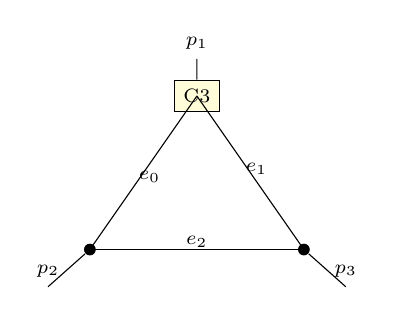
\begin{tikzpicture}[scale=.65,every node/.style={font=\scriptsize}]
\node[rectangle,draw,fill=yellow!15] (v0) at (3.27272727,4.18181818) {C3};
\node[circle,fill,inner sep=1.5pt] (v1) at (1.18181818,1.18181818) {};
\node[circle,fill,inner sep=1.5pt] (v2) at (5.36363636,1.18181818) {};
\draw[black] (3.27272727,4.18181818) .. controls (2.57575758,3.18181818) and (1.87878788,2.18181818) .. (1.18181818,1.18181818);
\node at (2.34660337,2.59864834) {$e_{0}$};
\draw[black] (3.27272727,4.18181818) .. controls (3.96969697,3.18181818) and (4.66666667,2.18181818) .. (5.36363636,1.18181818);
\node at (4.43751246,2.76498802) {$e_{1}$};
\draw[black] (1.18181818,1.18181818) .. controls (2.57575758,1.18181818) and (3.96969697,1.18181818) .. (5.36363636,1.18181818);
\node at (3.27272727,1.32727273) {$e_{2}$};
\draw (v0) -- (3.27272727,4.90909091) node[above] {$p_{1}$};
\draw (v1) -- (0.36363636,0.45454545) node[above] {$p_{2}$};
\draw (v2) -- (6.18181818,0.45454545) node[above] {$p_{3}$};
\end{tikzpicture}
\subsection*{G2}
% shared-layout-id: 4282a08670c031ee1950f4d00678242b8ed5798957f29456d184069d9b8b4d83
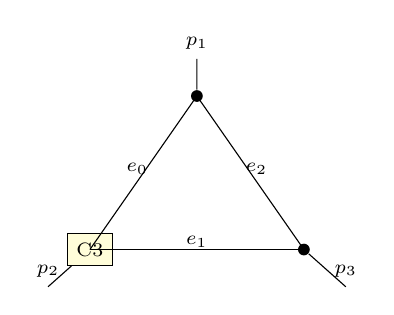
\begin{tikzpicture}[scale=.65,every node/.style={font=\scriptsize}]
\node[rectangle,draw,fill=yellow!15] (v0) at (1.18181818,1.18181818) {C3};
\node[circle,fill,inner sep=1.5pt] (v1) at (3.27272727,4.18181818) {};
\node[circle,fill,inner sep=1.5pt] (v2) at (5.36363636,1.18181818) {};
\draw[black] (1.18181818,1.18181818) .. controls (1.87878788,2.18181818) and (2.57575758,3.18181818) .. (3.27272727,4.18181818);
\node at (2.10794208,2.76498802) {$e_{0}$};
\draw[black] (1.18181818,1.18181818) .. controls (2.57575758,1.18181818) and (3.96969697,1.18181818) .. (5.36363636,1.18181818);
\node at (3.27272727,1.32727273) {$e_{1}$};
\draw[black] (3.27272727,4.18181818) .. controls (3.96969697,3.18181818) and (4.66666667,2.18181818) .. (5.36363636,1.18181818);
\node at (4.43751246,2.76498802) {$e_{2}$};
\draw (v1) -- (3.27272727,4.90909091) node[above] {$p_{1}$};
\draw (v0) -- (0.36363636,0.45454545) node[above] {$p_{2}$};
\draw (v2) -- (6.18181818,0.45454545) node[above] {$p_{3}$};
\end{tikzpicture}
\subsection*{G3}
% shared-layout-id: 86b69ef0c611a25f6e0e456b91c2adc284c301dbe992a69289aec0fcd8e7dcc1
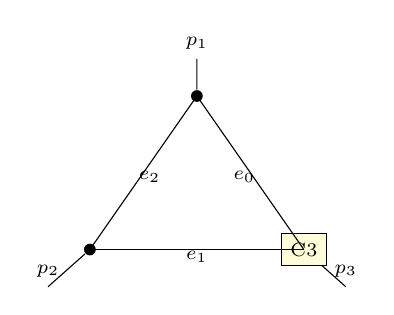
\begin{tikzpicture}[scale=.65,every node/.style={font=\scriptsize}]
\node[rectangle,draw,fill=yellow!15] (v0) at (5.36363636,1.18181818) {C3};
\node[circle,fill,inner sep=1.5pt] (v1) at (3.27272727,4.18181818) {};
\node[circle,fill,inner sep=1.5pt] (v2) at (1.18181818,1.18181818) {};
\draw[black] (5.36363636,1.18181818) .. controls (4.66666667,2.18181818) and (3.96969697,3.18181818) .. (3.27272727,4.18181818);
\node at (4.19885118,2.59864834) {$e_{0}$};
\draw[black] (5.36363636,1.18181818) .. controls (3.96969697,1.18181818) and (2.57575758,1.18181818) .. (1.18181818,1.18181818);
\node at (3.27272727,1.03636364) {$e_{1}$};
\draw[black] (3.27272727,4.18181818) .. controls (2.57575758,3.18181818) and (1.87878788,2.18181818) .. (1.18181818,1.18181818);
\node at (2.34660337,2.59864834) {$e_{2}$};
\draw (v1) -- (3.27272727,4.90909091) node[above] {$p_{1}$};
\draw (v2) -- (0.36363636,0.45454545) node[above] {$p_{2}$};
\draw (v0) -- (6.18181818,0.45454545) node[above] {$p_{3}$};
\end{tikzpicture}
\end{document}